\subsubsection{Experiments for Eliciting Happy Emotion}

To induce the emotion of happiness across different intensity levels, three separate tasks were designed. Each task corresponds to one of the three intensity levels: low, medium, and high. The tasks were chosen based on findings from psychological and affective computing literature that demonstrate the effectiveness of various stimuli for emotion elicitation.

\paragraph*{Low-Intensity Happiness – Watching a Funny Video}

The first task involved participants watching a short prank video clip titled “Circus Elephant Prank,” sourced from YouTube (\url{https://youtu.be/ZwJfXgTO7J4}) \citep{jls_pink_elephant}. This video features a light-hearted, humorous interaction involving a hidden elephant costume, designed to surprise and entertain pedestrians.

Studies show that visual stimuli, especially comedic videos, are highly effective for inducing happiness, as they generate strong self-reported emotions and physiological responses such as smiling and increased heart rate~\citep{emotionElictingsiedlecka2019}. Light-hearted content like animal pranks is typically perceived as safe and amusing, making it ideal for gently elevating mood without causing overstimulation.

The emotional intensity expected from such clips is generally low. Research indicates that cute or humorous videos involving animals or children tend to trigger emotions of low motivational intensity, which means the emotional state is pleasant but not highly arousing or action-driven~\citep{wang2022laugh}.

\paragraph*{Medium-Intensity Happiness – Autobiographical Recall}

For medium-intensity happiness, participants were asked to recall and verbally describe a recent event that made them feel happy. This task relies on autobiographical recall, a well-established emotion elicitation technique in psychological research.

Recollecting personal happy memories has been shown to increase both self-reported happiness and physiological responses such as heart rate~\citep{emotionElictingsiedlecka2019}. Moreover, autobiographical recall engages brain regions linked to reward processing, reinforcing the positive emotional experience~\citep{speer2017reminiscing}. This method is particularly meaningful because it draws from the participant’s own experiences, often resulting in a more personalized and emotionally moderate response compared to passive methods like video watching.

\paragraph*{High-Intensity Happiness – Playing a Game (Minesweeper)}

The third task was designed to evoke high-intensity happiness through a controlled gaming experience. Participants played a version of the classic puzzle game Minesweeper, which was modified to have a high probability of success—though this was not disclosed to the participant. Upon winning, the system delivered verbal praise and congratulations to enhance the reward experience.

Games, especially those that involve cognitive effort and strategic thinking, have been shown to elicit strong feelings of accomplishment and positive emotion~\citep{jones2014gaming}. Puzzle-based games like Minesweeper can be particularly rewarding when players succeed after investing effort, making them suitable for eliciting high-arousal positive emotions such as excitement and joy. By ensuring a high chance of winning, the task aimed to maximize the user’s feeling of success, thereby producing a more intense emotional response.

The screenshots related to happiness eliciting tasks are shown in Figure~\ref{fig:task-happy}. The first image shows the video clip, the second image shows the participant describing their happy memory, and the third image shows the Minesweeper game interface. The tasks were designed to be engaging and varied, ensuring that participants could experience happiness at different intensity levels.

\begin{figure*}[h]
    \centering
    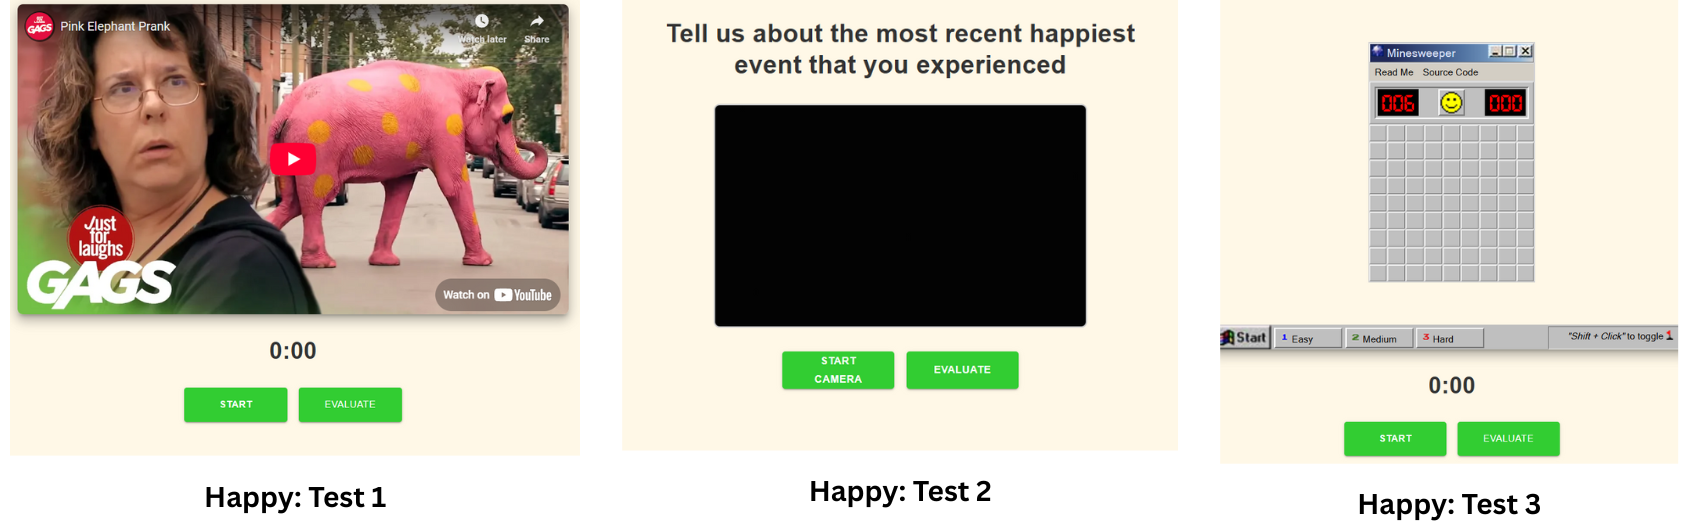
\includegraphics[width=1\textwidth]{img/chapter_03/happy_tests.png}
    \captionof{figure}{Eliciting tasks for Happy Emotion}
    \label{fig:task-happy}
\end{figure*}